%----------------------------------------------------------
\def\notedate{2021.11.14}
\def\currentauthor{Муха В. (РК6-73Б)}
%----------------------------------------------------------
\notestatement{rndhpcedt}{Первичный обзор литературы}

%----------------------------------------------------------
\subsubsection{Алгоритмы поиска циклов в графах}
Следующий материал является результатом анализа работы \cite{davidrajuh2016}.

\paragraph{Описание алгоритмов}
Существует несколько групп алгоритмов поиска:
\begin{enumerate}
    \item Алогритмы прохода
    \item Алгоритмы, основанные на матрице смежности
\end{enumerate}

Одним из представителей алгоритмов прохода является алгоритм depth-first-search (DFS). Сложность алгоритма $O(n^2)$ для одного прохода  $O(n^3)$ для всех проходов. Поэтому для ускорения алгоритма необходимо применение модификаций. \cite{Mahdi2011}
\newline\newline
Зададим граф $G(V, E)$, где $V$ - это множество вержин графа $(a, g)$, а $E$ - это множество граней графа $(ab, ad, ... , ge)$. Сам граф $G$ и его матрица смежности $A$ приведены ниже.
\begin{figure}[H]
	\centering
	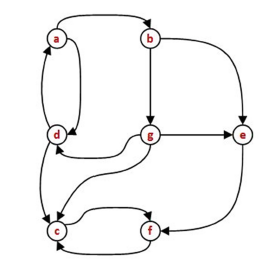
\includegraphics[width=0.3\textwidth]{ResearchNotes/rndhpc_not_edt_2021_11_14/adj_matrix.png}
	\caption{Граф и его матрица смежности} 
\end{figure}
Матрица смежности $A$ показывает, в какие узлы можно попасть из текущего, а транспонированная матрица $A^T$ показывает, из каких узлов можем попасть в текущий. 
Для того, чтобы определить циклы из двух шагов, нужно найти матрицу циклов $C$. Её можно найти, применив операцию AND над матрицами $A$ и $A^T$.
\begin{equation}
    C = (A \wedge A^T)
\end{equation}
Таким образом, матрица $C$ будет содержать все циклы из двух шагов. Для определения циклов из большего количества шагов необходимо применить операцию повторно.
%----------------------------------------------------------
\subsubsection{Поиск циклов в графах при помощи GPU}
Следующий материал является результатом анализа работы \cite{Mahdi2011}.

\paragraph{Проблема}
Поиск циклов в графе является NP-полной задачей, следовательно может быть выполнен за полиномиальное время.

\paragraph{Предложенное решение}
В статье приведен способ усорения поиска циклов с использованием GPU.

\paragraph{Описание решения}
Алгоритм работы следующий.
\begin{enumerate}
    \item Создаем новый массив узлов
    \item Для каждого узла параллельно создаём комбинацию для проверки
    \item При помощи алгоритма DFS(Depth First Search) находим циклы в каждом из потоков
    \item Повторяем алгоритм, пока не будут обнаружены все циклы
\end{enumerate}
%----------------------------------------------------------
% Атрибуты задачи
\noteattributes{}
%----------------------------------------------------------